% https://tex.stackexchange.com/a/445752
\documentclass{beamer}

\usepackage{tikz}
\usetikzlibrary{matrix,decorations.pathreplacing}
\pgfkeys{tikz/mymatrixenv/.style={decoration=brace,every left delimiter/.style={xshift=4pt},every right delimiter/.style={xshift=-4pt}}}
\pgfkeys{tikz/mymatrix/.style={matrix of math nodes,left delimiter=[,right delimiter={]},inner sep=1pt,row sep=0em,column sep=0em,nodes={inner sep=6pt}}}

\begin{document}
\begin{frame}[fragile]

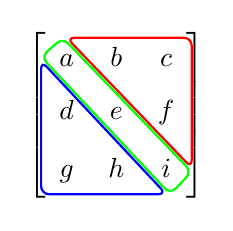
\begin{tikzpicture}[baseline=0cm,mymatrixenv]
    \matrix [mymatrix,text width=0.6em,align=center] (m)  
    {
    a & b & c \\ 
    d & e & f \\
    g & h & i \\
    };
    \pgfmathsetmacro{\offset}{0.5mm}
    \draw [thick,blue,rounded corners=1mm] (m-1-1.west) |- (m-3-3.south) -- cycle;
    \draw [thick,red,rounded corners=1mm] (m-1-1.north) -| (m-3-3.east) -- cycle;
    \draw [thick,green,rounded corners=1mm] ([yshift=\offset]m-1-1.west) -- ([xshift=-\offset]m-1-1.north) -- ([yshift=-\offset]m-3-3.east) -- ([xshift=\offset]m-3-3.south) -- cycle;
\end{tikzpicture}
\end{frame}

\end{document}
